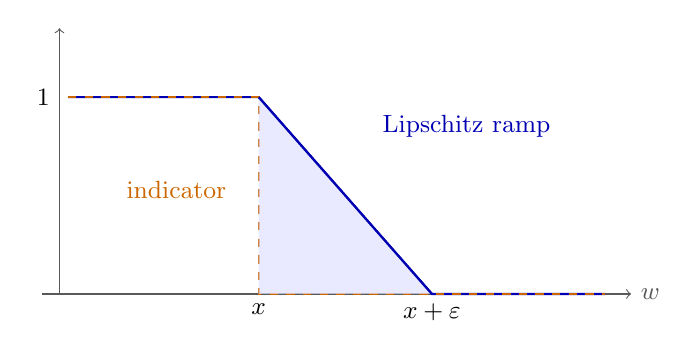
\begin{tikzpicture}[x=1.1cm,y=2.5cm]
\draw[->,black!65] (-2.5,0)--(4.3,0) node[right,font=\small] {$w$};
\draw[->,black!65] (-2.3,0)--(-2.3,1.35);
\draw[blue!70!black,thick] (-2.2,1)--(0,1)--(2,0)--(4,0);
\draw[orange!80!black,dashed,thick] (-2.2,1)--(0,1)--(0,0)--(4,0);
\fill[blue!12,opacity=0.7] (0,0)--(0,1)--(2,0)--cycle;
\draw[blue!70!black,thick] (0,1)--(2,0);
\node[left,font=\small] at (-2.3,1) {$1$};
\node[below,font=\small] at (0,0) {$x$};
\node[below,font=\small] at (2,0) {$x+\varepsilon$};
\node[font=\small,blue!70!black] at (2.4,0.85) {Lipschitz ramp};
\node[font=\small,orange!80!black] at (-0.95,0.53) {indicator};
\end{tikzpicture}
